\documentclass[11pt,a4paper]{article}
\pdfinfoomitdate=1
\pdftrailerid{}
\pdfsuppressptexinfo=15
\usepackage[T1]{fontenc}
\usepackage[utf8]{inputenc}
\usepackage{lmodern,microtype}
\usepackage[a4paper,margin=24mm,headheight=15pt]{geometry}
\usepackage{amsmath,amssymb,booktabs,tabularx,longtable,array,graphicx}
\usepackage[table]{xcolor}
\usepackage{tikz}
\usetikzlibrary{arrows.meta,positioning,calc}
\usepackage{enumitem,fancyhdr,float,caption,url}
\usepackage[numbers,sort&compress]{natbib}
\usepackage[colorlinks=true,linkcolor=purple,citecolor=purple,urlcolor=purple,breaklinks=true]{hyperref}
\definecolor{FoundryPurple}{HTML}{382062}
\definecolor{FoundryLilac}{HTML}{F1EDF8}
\definecolor{FoundryInk}{HTML}{20212A}
\definecolor{FoundryTeal}{HTML}{116E71}
\definecolor{FoundryAmber}{HTML}{9B5C10}
\color{FoundryInk}
\hypersetup{pdftitle={AGI ALPHA FLYWHEEL: The Software Capability Foundry},pdfauthor={MONTREAL.AI},pdfsubject={Prospective bounded software capability construction and reuse}}
\setlist{itemsep=2pt,topsep=4pt,leftmargin=*}
\setlength{\parskip}{4pt}
\setlength{\parindent}{0pt}
\setlength{\emergencystretch}{2em}
\renewcommand{\arraystretch}{1.18}
\captionsetup{font=small,labelfont=bf}
\pagestyle{fancy}
\fancyhf{}
\fancyhead[L]{\small\color{FoundryPurple}AGI ALPHA FLYWHEEL}
\fancyhead[R]{\small Software Capability Foundry}
\fancyfoot[L]{\scriptsize Independent research edition 1.0 \textbullet\ 25 October 2026}
\fancyfoot[R]{\thepage}
\newcommand{\code}[1]{\texttt{\small #1}}
\newcommand{\status}[1]{\textbf{\color{FoundryPurple}#1}}
\newcommand{\AbstractResult}{All 1,344 outputs qualify, and the flywheel produces 96 verified selected-parent diagnostic invocations across 24 generated instances. Its geometric mean whole-instance CPU ratio to the direct specialist is 1.0574 (95\% interval 1.0246--1.0899), failing the preregistered superiority gate.}
\newcommand{\ConclusionResult}{The practical batching improvement survives exact output checks, while the proposed flywheel does not outperform the direct specialist after measured pipeline costs. Useful reusable engineering is demonstrated; a superior improvement process is not.}

\begin{document}
\thispagestyle{empty}
{\sffamily\small\bfseries\color{FoundryPurple} AGI ALPHA FLYWHEEL \hfill $\infty$}
\vspace{7mm}

{\sffamily\fontsize{30}{34}\selectfont\bfseries\color{FoundryPurple}
The Software\\Capability Foundry\par}
\vspace{4mm}
{\Large From Verified Improvements\\to Better Means of Improving\par}
\vspace{5mm}
{\sffamily\bfseries SUCCESSOR $\Omega$ HARNESS\quad ACTIVATE. EVOLVE. SCALE.\par}
{\small Powered by TRANSFORMATIONAL INTELLIGENCE $\infty$\par}
\vspace{5mm}
\textbf{MONTREAL.AI}\quad Research direction: Vincent Boucher\\
Independent research edition 1.0\quad 25 October 2026

\vspace{5mm}
\begin{abstract}
\noindent An autonomous improvement system should leave behind a better means of doing the next useful job. That claim requires more than a fast patch: a retained instrument must transfer, help form a distinct later capability, and justify its complete cost against competent alternatives. We study a concrete source-verification bottleneck in the public AGI ALPHA ecosystem. A bounded Git snapshot reader replaces repeated per-file processes while preserving exact committed bytes, regular-file and size checks, and original downstream output checks. It transfers from companion-package verification to gallery-worker reconstruction. A deterministic constructor then binds the accepted reader into a distinct archive-drift diagnostician. A prospective campaign freezes source, comparators, generation rules, budgets and analysis before creating 24 fresh source-derived repository instances. Seven treatments include a direct native specialist, an asset-free capable controller, ordinary saved tooling, an equally enabled conventional builder, the proposed flywheel, an independently written equivalent, and exact reconstruction. \AbstractResult{} Complete research investment, monetary payback, autonomous algorithm discovery and acceleration remain unestablished. The contribution is an executed, auditable separation of useful engineering, capability transfer and improvement-process claims, with reviewable patches, raw failures, an existing-workbench browser demonstration and a complete reproduction package.
\end{abstract}
\vspace{2mm}
\colorbox{FoundryLilac}{\parbox{\dimexpr\textwidth-2\fboxsep}{\small
\textbf{Evidence boundary.} Deterministic local research and browser computation were executed. Production release approval, an approved external executor, live Jobs settlement and economic authority are separate and are not inferred.}}
\vfill
\textbf{Make the next turn worth taking.}\hfill\small\href{https://github.com/MontrealAI/AGI-Alpha-Agent-v0/issues/4850}{Research coordination and evidence}
\clearpage

\section{The next turn should inherit a better means}
\label{sec:introduction}

Software maintenance repeatedly pays for the same kinds of work: locating committed inputs, reconstructing dependency information, preparing evidence, and explaining why a result is safe to use. An optimization can remove one such cost. A more consequential outcome is a qualified engineering instrument that helps another maintainer make a different improvement. The central question is whether this retained instrument improves fresh work after the costs of discovering, constructing, checking, integrating and maintaining it are included.

\begin{quote}
\textbf{Build software that improves useful software, and leaves behind better means of making the next improvement.}
\end{quote}

The Software Capability Foundry examines that question through \emph{qualified boundaries as reusable engineering assets}. A boundary separates the implementation that may change from the externally required behavior that must remain valid. Its value is practical: a later constructor can use a well-defined operation without reconstructing every implementation decision, while a verifier can determine when that operation is no longer applicable. The asset is therefore executable code together with a checked contract, provenance, resource account, failure behavior and a way back to the incumbent. A saved answer or a successful benchmark row does not provide this interface.

The immediate setting is repository and publication tooling in the public AGI ALPHA ecosystem. Repeated short-lived tool invocations are a plausible source of overhead, but invocation count alone is not a performance result. The study begins with pinned source call sites and reproduces their required outputs in disposable local repositories. It distinguishes useful restructuring of the computation from a relaxation of checks. For example, changing how committed bytes are acquired must preserve which revision, object type and content the caller receives; skipping a release-integrity check would change the mission.

\subsection{Three achievements require three tests}

We distinguish a \emph{service improvement}, a \emph{transferable capability}, and an \emph{improved improvement process}. The first delivers a useful result at lower justified burden. The second helps on a fresh problem with changed inputs or structure. The third reduces the complete work needed to discover or qualify a further improvement. These implications do not follow automatically. Reusing a fast function may establish the second without establishing the third. A child program that imports a parent without benefiting from it establishes neither.

The visible journey contains four predeclared missions. Mission A delivers a useful improvement and retains its engineering interface. Mission B changes the workload and tests that interface's contribution. Mission C uses accepted prior work to help construct or qualify a distinct capability with a different output contract. Mission D changes the operating conditions enough that reuse must be refused, replaced or requalified. These explanatory missions remain separate from the protected confirmation instances.

The decisive comparisons concern useful content rather than lineage terminology. Removing the parent still permits reconstruction from legitimate knowledge and ordinary repository history. An independently constructed equivalent asset tests whether any benefit belongs to the asset's content. A mature specialist and an equally enabled conventional tool builder remain eligible to win. This follows the baseline and evidence-package discipline of AGI ALPHA rather than treating a new label as a privileged comparator~\cite[PDF pp.~37, 60, 69]{agi_alpha}.

\subsection{Why the earlier failures matter}

The preceding research supplies useful mechanisms and reasons for stricter comparisons. The Possibility Foundry constructed a reusable instrument and used it in a distinct temporal capability, but an analytical specialist and an independent construction policy found the same instrument more cheaply. Charging the complete ancestor search to the small successor campaign also reversed its affordability~\cite[PDF pp.~2--4]{possibility_foundry}.

The published coordination record for Strategy Succession reports 517 qualified missions out of 864 for the primary flywheel, tied with the equally enabled learner and below the stronger portfolio's 591. No primary retained capability was admitted; no fresh repair output both invoked its parent and qualified. Its diagnostic inheritance advantage against exact reconstruction disappeared against a cheaper conventional fallback~\cite{strategy_record}. The subsequent \emph{Earn the Next Turn} record reports constructive succession and parent-invoking fresh outputs, while its whole-participant CPU comparison failed the predeclared five-percent admission margin against native factor reuse and refactorization~\cite{earned_turn_record}. These are preserved prior results, not observations from the new experiment.

Those findings motivate a narrower and more demanding contribution. The present study asks an engineering asset to survive a competent alternative, a current correctness check, complete participant accounting and an explicit changed-scope case. It does not force parent reuse when a cheaper direct method works. Service resources and improvement resources are recorded separately, so unsuccessful research does not silently consume the resources promised for the useful delivery.

\subsection{Scope of the contribution}

The experiment studies bounded deterministic construction and qualification. Its primitive tools and candidate mechanisms are supplied and disclosed. Any optimization found within that space is a result about the executed search and selected artifact; it is not evidence of general autonomous invention. The browser experience makes the goal, result, retained interface, comparison and decision inspectable, while distinguishing live local computation, recorded experiment evidence and execution through an approved external adapter.

The work is additive to the existing workbench and mission history. It introduces no production scheduler and derives no execution authority from a research result. The empirical report must answer two separate questions: whether the capability is worth using on the next specified mission, and whether its complete investment has paid for itself. Unknown monetary or human costs remain unknown. A reliable reduction in engineering burden can be useful without demonstrating cash profit, open-ended compounding or an increasing rate of improvement.

\section{Technical foundations and implemented interpretation}
\label{sec:foundations}

The foundational papers supply specific design obligations. Their theoretical examples, architectural proposals and prior measured results do not certify this implementation. The source audit records the exact public PDF bytes and 1-based PDF page locations used below.

\subsection{Preserve the purpose; change the engineering means}

Transformational Intelligence separates the authorized intent charter, the problem formulation and the evaluation instrument. A proposed transformation contains an executable construction, a realization in the original environment, and a witness identifying the restriction changed and the evidence that could refute its advantage~\cite[PDF pp.~3, 7--8]{transformational_intelligence}. Here the preserved purpose is the caller's required repository or publication result. The mutable means are decomposition, batching, instrumentation and reusable interfaces. The final correctness oracle is outside the candidate's editable mechanism. A defect in that oracle requires an explicit correction and a new evidence boundary; it cannot be repaired invisibly after a disappointing result.

\emph{Out-Learn} makes a measurement protocol and its calibration into constructed objects. Its reuse horizon changes the rational up-front investment, and a changed nuisance class can invalidate the query program without invalidating every historical calibration~\cite[PDF pp.~7, 12--14]{out_learn}. The engineering analogue is a portable instrument with an explicit measurement contract: which runtime is measured, which preparation work is included, which caches are controlled, and which changes require remeasurement. Timing variability is reported rather than canceled by assertion.

\emph{Out-Think} requires a representation to support future operations as well as current answers. Its finite-state constructor closes distinguishing obligations under those operations; an added operation can invalidate the compact representation~\cite[PDF pp.~4, 12--13]{out_think}. The retained engineering interface consequently records relevant object semantics and failure conditions, not merely an attractive timing summary. This analogy does not transfer a finite-state theorem to an arbitrary filesystem: actual input and object behavior still require direct checks.

\subsection{Make the boundary useful to another constructor}

\emph{Out-Execute} supplies the closest mechanism. In its finite factor model, a component may change internally without forcing external optimization to change when its complete boundary value function remains identical. A current internal witness is still required, and current-output acceptance is retained~\cite[PDF pp.~5--8, 11]{out_execute}. We apply the engineering principle: preserve the caller-visible contract while changing the implementation beneath it, then make that operation available to a later constructor. No general claim that arbitrary tests can be skipped follows. A valid digest identifies bytes; it does not independently establish the semantics of the program that produced them.

\emph{Out-Strategise} distinguishes an installed asset, retained uncertainty and a purpose-specific abstraction. They have different expiry conditions. A stronger archive can improve performance even when the discovery policy is unchanged, so a claim about improved discovery must separate archive content from construction policy~\cite[PDF pp.~12--14]{out_strategise}. This motivates the removed-parent, reconstruction and equivalent-asset comparisons. Parent ancestry is not the treatment of scientific interest when the same useful content can be constructed conventionally.

\emph{Out-Evolve} asks the first capability to support fresh purposes and then help construct a different capability. Its retained object contains an executable realization, semantic or empirical contract, operating envelope, resource account and legitimate access~\cite[PDF pp.~6--8, 14]{out_evolve}. Mission C targets this construction link. A distinct interface and accepted function are necessary, while a parent-invocation trace establishes which prior bytes actually contributed. They do not alone prove that the resulting construction process beats equally capable alternatives.

The Possibility Foundry gives an executed precedent for keeping these claims separate. Its constructed instrument expanded a defined affordable work set, yet cheaper builders selected identical content; its successor's marginal feasibility did not imply recovery of all ancestor costs~\cite[PDF pp.~2--4]{possibility_foundry}. The present comparison therefore retains both the strongest direct method and ordinary reusable engineering as live alternatives.

\subsection{Account for resources that can actually be reused}

\emph{Out-Design} defines a release certificate that connects preserved service behavior to capacity freed at a usable location. Its successor adds a different service rather than merely rearranging old ones~\cite[PDF pp.~5, 12--13]{out_design}. For software, this motivates a stricter feedback test than multiplying nominal saved seconds by an assumed price. A measured saving must be available within the relevant execution envelope, allocated to a bounded follow-up task, and accompanied by a record of the useful work that task produced. CPU time, wall time, process count, bytes, runner occupancy and money remain separate quantities. Externally supplied research resources are not relabeled as earnings.

AGI ALPHA's Evidence Docket and capability-package requirements make these accounts inspectable. They bind environment, tasks, baselines, execution, proof bundles, costs, lineage, replay and rollback~\cite[PDF pp.~37, 60, 69]{agi_alpha}. The new study uses that evidence structure for an engineering contribution. It does not inherit the broader architecture's scaling, financial or deployment claims.

\subsection{Freeze evidence; preserve existing authority boundaries}

Mission-Sovereign Successor freezes the mission, strongest credible alternative, complete burden denominator and stop-loss before protected comparison. Its fresh-successor gate binds one challenger and uses matched outcomes with a lower-confidence requirement plus hard gates~\cite[PDF pp.~32, 41]{mission_sovereign}. Mission Gym separately represents rewards and noncompensable constraints, caps formation search, and keeps development feedback distinct from promotion evidence~\cite[PDF pp.~19, 38, 40, 48]{gym_specialist}. In this study, these ideas become frozen configurations, separate service and improvement accounts, a fixed confirmation boundary, incumbent retention and typed refusal.

Neural-Symbolic SUCCESSOR~$\Omega$ requires the release manifest to declare permitted learning and writable state. Its Chronicle preserves history without treating history as proof. It also distinguishes internal review from externally independent custody~\cite[PDF pp.~17, 26--28, 30]{neural_symbolic_v1}. A separate assistant reviewer is disclosed as internal separation; common authorship, provider and environment remain possible sources of correlated error. No claim of external institutional validation follows.

SUCCESSOR~$\Omega\times$AGI Jobs expresses work as typed, sealed contracts with input scope, tools, budgets, acceptance, evidence and rollback. Its refinement relation forbids a lower-burden implementation from weakening hard guarantees or provenance. Its runtime proposal separates execution, verification, admission and authority~\cite[PDF pp.~16--19, 54, 71, 82--83]{successor_jobs}. The implementation uses eligible existing workbench and export interfaces where available. A browser mission pack, an unsigned draft, a local receipt and an approved executor run are different evidence states. This study invokes no deployed financial contract and claims no live settlement or activated token utility.

\paragraph{Operational stage map.}
\textbf{Identify} fixes the useful result and recurring obstruction; \textbf{Out-Learn} measures the bottleneck under a declared protocol; \textbf{Out-Think} chooses a sufficient reusable representation; \textbf{Out-Design} constructs an equivalent implementation; \textbf{Out-Strategise} decides whether building and retaining it are justified; \textbf{Out-Execute} delivers with current correctness and recovery evidence; \textbf{Out-Evolve} tests fresh reuse and construction of a distinct later capability. These labels organize the recorded work. The evidence for each transition remains its actual program, receipt and comparison.


\section{The software boundary and the real baseline}
\label{sec:baseline}

The starting point is a read-only audit of four public repositories. Table~\ref{tab:pins} identifies the exact snapshots; the companion contains full 40-character identities, retrieved instructions, workflow observations and source hashes. These snapshots are not interchangeable with installed or deployed releases. Alpha's main snapshot includes the Strategy Succession implementation, while the contemporaneous coordination record keeps its 1.44 release unqualified and unpublished. The prior 1.43 release and the existing release owner are preserved. Original Harness and Fleet holds are not retried or transferred to this study.

\begin{table}[htbp]\centering\small
\caption{Pinned audit snapshots. Abbreviations are for readability; the evidence manifest records exact commits.}
\label{tab:pins}
\begin{tabularx}{\textwidth}{@{}l l X@{}}\toprule
Repository & Commit prefix & Role in this study\\\midrule
AGI-Alpha-Agent-v0 & \code{f836f06e8351} & Actual verification hot spots and unchanged browser workbench\\
AGIJobsv0 & \code{bc4abbd5c28f} & Source and release-policy inspection only\\
AGIJobManager & \code{5d5670df9dbb} & Source and release-policy inspection only\\
AGI-Fleet-Linux & \code{45759fb096fa} & Adapter and held-operation inspection only\\\bottomrule
\end{tabularx}
\end{table}

The eligible development portfolio is small and purpose-driven. Mission A retrieves the exact source bodies required to validate the Strategy companion. The original \code{\_committed\_files} reads its configuration, enumerates the declared package payload and launches a fresh Git process for each body. The audited inventory contains 37 files and 456,459 bytes; configuration is retrieved twice, giving 39 processes including the tree listing. The intended user is the release operator who must confirm that the package is built from the accepted source.

Mission B reconstructs gallery service-worker outputs from committed cache inputs. The original \code{paper\_changes.expected\_workers} reads one catalog and 437 assets totaling 16,135,527 bytes through separate size and body calls. This entails 876 Git subprocesses, excluding the already acquired tree. This operation is invoked for both sides of a paper transition. The surrounding history proof may repeat it across transitions. That source-level recurrence explains why the bottleneck is worth investigating; no assumed frequency is converted into a realized saving.

Mission C constructs a complete archive-drift report: which expected paths are missing, which present paths changed, and which paths are unexpected. This is a different interface and output contract from retrieval. It can reduce repeated investigation of an invalid artifact without turning diagnosis into release acceptance. Mission D introduces unsupported identities, paths, modes, corrupted objects or unsafe archives and requires refusal. The portfolio excludes dependency installation and test-impact analysis, whose broader correctness and environment costs would not fit this bounded experiment.

Historical CI outcomes are diagnostic context only. The study does not claim that the old full CI runtime measures the new patch's effect, and it does not remove tests, platforms, security scans or release checks. A valuable strong baseline already exists: \code{accept\_public\_strategy.core\_payload} checks archive body identities in process. We therefore do not describe that function as a per-member process bottleneck.

\subsection{Representation change}

The underlying transformation replaces a sequence of short-lived body queries with a bounded stream of immutable Git object bodies. Requested paths are resolved in an exact commit; modes, object kinds and sizes are inspected; object IDs are deduplicated; a batch command retrieves the bodies; and every returned body is checked against its Git blob identity. A SHA-256 output inventory supplies an additional evidence identity. Deduplication is confined to immutable object IDs in one call. No persistent result is trusted because a mutable file has an unchanged size or modification time.

This uses documented Git batch and tree interfaces~\cite{git_cat_file,git_ls_tree}, not a novel optimization algorithm. The proposed research contribution concerns how the operation is retained, applied, constructed into a distinct instrument and evaluated against strong reuse alternatives. Both the proposed reader and the independently written specialist use two Git processes for a generic inventory. The caller adaptations may require multiple bounded reads: configuration first, followed by its exact declared payload. The original caller's mode restrictions remain intact; a general reader accepting executable regular files does not widen the paper-only caller's non-executable-file policy.

\section{Capabilities with executable boundaries}
\label{sec:assets}

An eligible retained asset is a tuple
\begin{equation}
  A=(b,v,I,D,P,L,Q,M,R),
\end{equation}
where $b$ is executable content, $v$ its version, $I$ its interface, $D$ its dependency closure, $P$ its provenance, $L$ its operating limits, $Q$ its qualification evidence, $M$ its maintenance account, and $R$ its rollback behavior. Unknown components of $M$ are represented as unknown, not zero. Neither a filename nor a lineage label supplies qualification.

The reader's interface is \code{read(repo, commit, paths, max\_file, total)}. The default contract accepts 1--256 unique canonical relative POSIX paths, an exact 40-hex SHA-1 commit, ordinary regular blob modes, files no larger than 8 MB and at most 32 MB of requested bodies. It rejects symbolic links, gitlinks, directories, mutable references, missing paths, invalid names, invalid limits, and detected object corruption. Callers with a separately qualified larger per-file policy pass that policy explicitly and chunk large inventories without omitting a member.

The trust boundary remains a local Git repository and Git's interpretation of the commit/tree graph. The reader recomputes blob identities; it is not a separate implementation of Git object-database authentication. Existing source, release, signature and security checks remain required. SHA-1 object identity is inherited from the pinned repository format and is not represented as a new release-signing guarantee.

\begin{figure}[t]
\centering
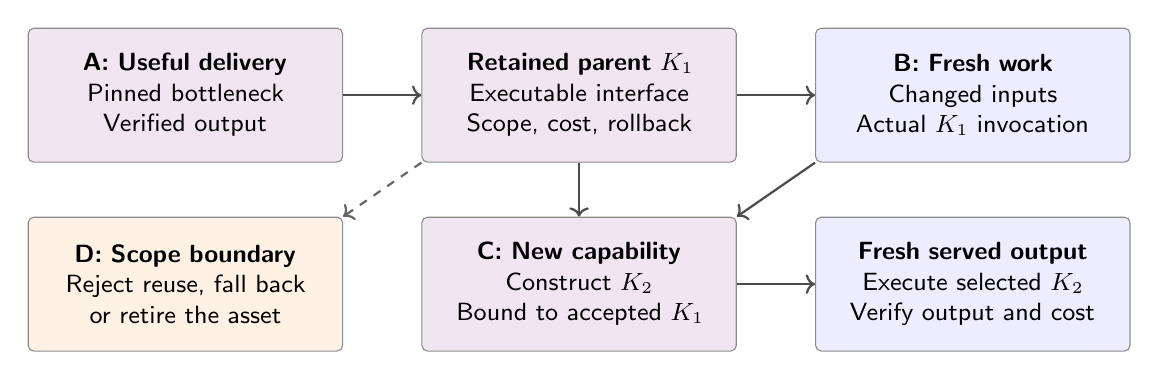
\begin{tikzpicture}[
  font=\sffamily\small,
  box/.style={draw=black!45, rounded corners=2pt, align=center, text width=3.5cm, minimum height=1.7cm, inner sep=7pt},
  flow/.style={->, thick, draw=black!70},
  guard/.style={->, thick, dashed, draw=black!60}
]
\node[box,fill=violet!10] (a) at (0,0) {\textbf{A: Useful delivery}\\Pinned bottleneck\\Verified output};
\node[box,fill=violet!10] (k) at (5,0) {\textbf{Retained parent $K_1$}\\Executable interface\\Scope, cost, rollback};
\node[box,fill=blue!7] (b) at (10,0) {\textbf{B: Fresh work}\\Changed inputs\\Actual $K_1$ invocation};
\node[box,fill=violet!10] (c) at (5,-2.4) {\textbf{C: New capability}\\Construct $K_2$\\Bound to accepted $K_1$};
\node[box,fill=blue!7] (serve) at (10,-2.4) {\textbf{Fresh served output}\\Execute selected $K_2$\\Verify output and cost};
\node[box,fill=orange!10] (d) at (0,-2.4) {\textbf{D: Scope boundary}\\Reject reuse, fall back\\or retire the asset};
\draw[flow] (a) -- (k);
\draw[flow] (k) -- (b);
\draw[flow] (k) -- (c);
\draw[flow] (b.south west) -- (c.north east);
\draw[flow] (c) -- (serve);
\draw[guard] (k.south west) -- (d.north east);
\end{tikzpicture}
\caption{Artifact lineage and failure boundary. A useful delivery, fresh reuse and construction of a distinct capability are separate achievements. The child must be tied to accepted parent bytes, and the selected child must actually use them when required by the claimed mechanism. Scope failure preserves the history while ending the invalid reuse claim.}
\label{fig:lineage}
\end{figure}


The child constructor writes executable Python bytes, records a version and dependency closure, and binds the selected parent's SHA-256 to the acceptance record of the actual earlier read. A child call verifies the parent source, invokes its reader, compares a bounded captured ZIP against the resulting committed bodies, and emits all three drift sets. The acceptance record is a local evaluator-issued research record, not a signed production admission credential; the constructor assumes trusted issuance. The selected-execution trace contains the parent identity, acceptance-record identity, commit, input-path digest and output-inventory digest. The outer evaluator checks these values against its own oracle.

ZIP capture rejects duplicate and unsafe names, NUL truncation, directory or symbolic-link entries, encrypted members, unsupported compression, bad CRCs, and size expansion beyond the declared limits. Capture checks an opened regular-file descriptor and detects changes during the read. An empty ZIP is a valid diagnostic input: all expected files are reported missing. No archive is extracted and no source file is changed. The output helps an operator investigate; it does not authorize replacing or publishing an artifact.

The constructor is intentionally finite. It composes a prewritten reader interface with a prewritten drift comparison and current acceptance binding. It does not invent the drift algorithm from Mission B's contents. Accepted B work determines the starting asset identity; the distinct C output contract is predeclared. This establishes a concrete executable succession path if it qualifies, while leaving autonomous invention and improved discovery policy as separate hypotheses.

\section{Prospective experiment}
\label{sec:experiment}

Development compares three supplied retrieval methods and one child template. The original unmodified call site is also timed as a delivery baseline. The reader selection uses five interleaved Mission A trials and median total CPU among correct eligible methods. The selected method is then applied to Mission B without tuning on B. All prefreeze implementation corrections and the independent specialist's initial three-process version are disclosed in the development ledger. The finite grammar is not described as the complete number of engineering attempts.

Before confirmation, the study freezes the reader, specialist, constructor, child comparison, worker, measurement code, campaign runner, statistical analysis, independent oracles, task generator, selected source, protocol and environment description. A fresh 256-bit seed is generated only after this boundary. A disclosed prospective storage-only amendment preserves the original freeze and identical scientific file map: automatic approval review blocked durable checkpoint saving, so authorized local execution continued with a hash-verified local checkpoint. No confirmation task or result existed before that amendment; durable saving remained a separate pending action. The task generator has not been executed during development. A separately recorded task lock binds the generated case manifest, archive bytes and oracle documents before the first candidate worker. Both source and task identities are checked again after the campaign.

\subsection{Protected cases and experimental units}

The generator selects a fixed pool of public source bodies from the pinned Alpha snapshot, excluding the earlier study directories and Strategy companion. It constructs 24 new Git repositories with inventories of 8, 24, 64 or 128 files, changed directory depth, spaces, Unicode names and regimes with repeated content. The working trees are deliberately poisoned after commit so a filesystem shortcut cannot accidentally satisfy the oracle. Archive cases are prospectively assigned clean, changed, missing, extra, or combined drift. Expected byte hashes and drift sets are computed during fixture construction without importing candidate code.

These are 24 generated repository instances in one source ecosystem. They are not 24 naturally sampled projects or independent organizations. The statistical unit is the generated instance; repeated operations within one instance are aggregated before inference. Conclusions are conditional on this source pool, generator, software environment and host. The source bodies are genuine public software; the layouts and defects are controlled experimental constructions. The package makes that distinction inspectable.

\subsection{Seven strong treatments}

\begin{table}[htbp]\centering\small
\caption{Comparator rights and executed behavior. All treatments receive the same task information, legitimate method sources, functional correctness, scope and budget requirements. Constructed-child arms additionally require the mechanism-specific parent trace.}
\label{tab:arms}
\begin{tabularx}{\textwidth}{@{}l X@{}}\toprule
Treatment & Permitted implementation\\\midrule
Specialist & Independently authored two-process native reader and direct complete drift diagnosis; available from the start.\\
No asset & Same capable deterministic controller without the proposed serialized parent; may use the specialist directly and does not pay an artificial reconstruction penalty.\\
History & Ordinary saved selected tooling plus direct drift comparison, without a newly constructed child artifact.\\
Conventional & Equally enabled reusable-tool constructor with the same grammar, source access, budgets and child template as the flywheel.\\
Flywheel & Retained selected reader, accepted fresh read, then an executable child bound to that acceptance record.\\
Equivalent & Independently implemented equivalent reader content, with the same child template and current qualification.\\
Reconstruction & Rebuild the selected reader artifact from its legitimate supplied source, then qualify and construct the child.\\\bottomrule
\end{tabularx}
\end{table}

The conventional and flywheel treatments deliberately share the construction mechanism. Their distinction does not create an information or budget advantage. The comparison tests whether the proposed label has any experimentally identifiable advantage beyond ordinary content reuse. Similarly, the no-asset treatment can retain a competent direct specialist; removing an artifact is not a license to remove useful knowledge. Reconstruction retains access to legitimate source templates, making it a strong practical intervention rather than amnesia.

\begin{figure}[t]
\centering
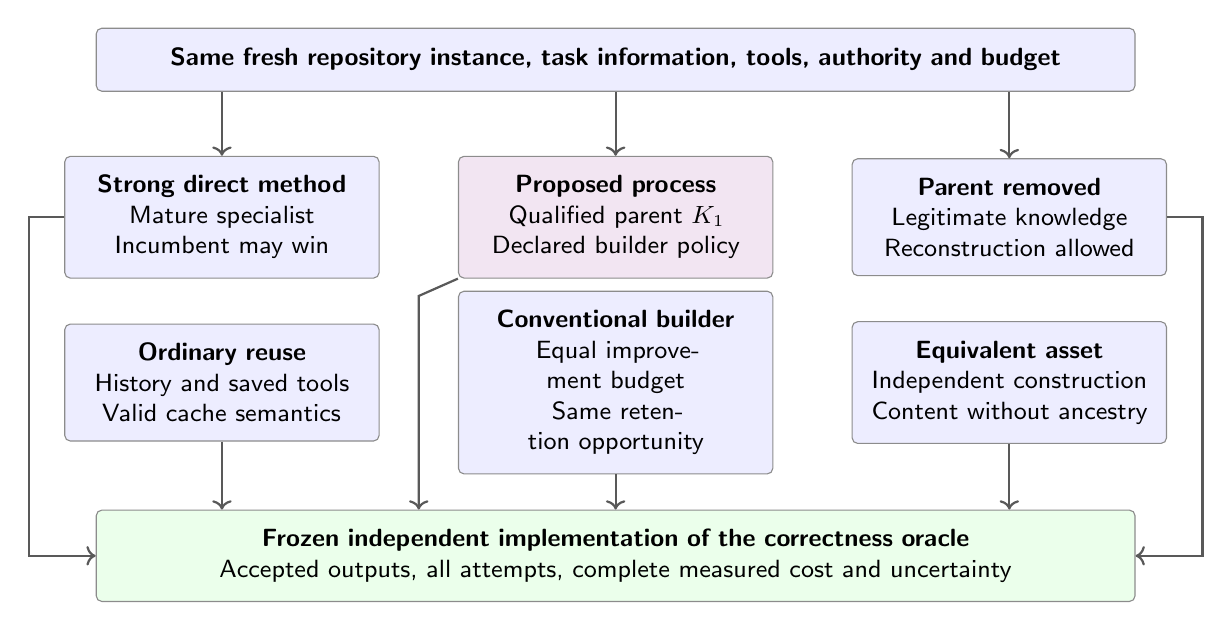
\begin{tikzpicture}[
  font=\sffamily\small,
  box/.style={draw=black!45, rounded corners=2pt, align=center, text width=3.5cm, minimum height=1.15cm, inner sep=7pt},
  flow/.style={->, thick, draw=black!65}
]
\node[box,fill=blue!7,text width=12.7cm,minimum height=0.8cm] (inputs) at (5,0) {\textbf{Same fresh repository instance, task information, tools, authority and budget}};
\node[box,fill=blue!7] (direct) at (0,-2) {\textbf{Strong direct method}\\Mature specialist\\Incumbent may win};
\node[box,fill=violet!10] (parent) at (5,-2) {\textbf{Proposed process}\\Qualified parent $K_1$\\Declared builder policy};
\node[box,fill=blue!7] (removed) at (10,-2) {\textbf{Parent removed}\\Legitimate knowledge\\Reconstruction allowed};
\node[box,fill=blue!7] (ordinary) at (0,-4.1) {\textbf{Ordinary reuse}\\History and saved tools\\Valid cache semantics};
\node[box,fill=blue!7] (conventional) at (5,-4.1) {\textbf{Conventional builder}\\Equal improvement budget\\Same retention opportunity};
\node[box,fill=blue!7] (equivalent) at (10,-4.1) {\textbf{Equivalent asset}\\Independent construction\\Content without ancestry};
\node[box,fill=green!8,text width=12.7cm,minimum height=1.0cm] (judge) at (5,-6.3) {\textbf{Frozen independent implementation of the correctness oracle}\\Accepted outputs, all attempts, complete measured cost and uncertainty};
\foreach \n in {direct,parent,removed}{\draw[flow] (inputs.south -| \n.north) -- (\n.north);}
\draw[flow] (direct.west) -- ++(-0.45,0) |- (judge.west);
\draw[flow] (parent.south west) -- (2.5,-3.0) -- (2.5,-5.2) -- (judge.north -| 2.5,0);
\draw[flow] (removed.east) -- ++(0.45,0) |- (judge.east);
\foreach \n in {ordinary,conventional,equivalent}{\draw[flow] (\n.south) -- (judge.north -| \n.south);}
\end{tikzpicture}
\caption{Causal comparison structure. Parent removal measures the value of ready executable content while permitting reconstruction. An equivalent asset distinguishes content from ancestry. Ordinary reuse and an equally funded conventional builder prevent attributing familiar engineering advantages to a new name. Repeated timings within an instance are subsamples, not additional independent missions.}
\label{fig:comparisons}
\end{figure}


\subsection{Execution, costs and admission}

Every instance/treatment pair executes a fresh Python read worker with four reads, then a fresh child worker with four diagnoses. Within each phase, the first call is labeled fresh-process and three subsequent calls warm-process. The operating-system page cache is shared and not flushed; no physical disk-cold claim is made. The order of the 168 instance/treatment pairs is randomized. Python 3.12.14 and Git 2.51.1 run on the recorded Linux x86-64 host with nine visible CPUs. Concurrent host load is not controlled, which motivates interleaving and uncertainty reporting.

Service and improvement ledger entries are distinct. A worker has a hard 30-second wall timeout. Per-instance service and improvement sums have separate 20-second and 10-second admission caps; they are postmeasurement admission limits, not kernel CPU quotas. Timeout and malformed-output attempts remain failed, charged outcomes. A failed read prevents child construction. Separate ledger accounts and postmeasurement admission caps do not establish protected operational resource reservation or preemptive enforcement of a promised service budget. Such enforcement remains untested. Source does not receive or modify the final oracle; the outer runner checks B outputs before providing the content-bound acceptance receipt used for C.

The primary cost is total parent-plus-completed-child CPU for each full instance/treatment sequence, including worker startup, artifact materialization, child construction, retrieval, output verification and intermediate evidence persistence. The final summary-row write and common source/task setup are reported separately from that estimand. Parent CPU, child CPU and wall time remain distinct in raw records. Four repetitions are not treated as four independent trials.

For instance $i$, let $C_{i,F}$ and $C_{i,S}$ be flywheel and specialist costs. The primary estimator and prespecified gate are
\begin{align}
 \widehat{\rho}&=\exp\!\left(\frac{1}{24}\sum_{i=1}^{24}\log\frac{C_{i,F}}{C_{i,S}}\right),\\
 \mathrm{admit}&=\mathbf{1}\{\text{all required checks pass}\}\,
                  \mathbf{1}\{U_{0.95}(\rho)<0.95\}.
\end{align}
The 95\% percentile interval uses 10,000 paired instance bootstrap resamples with a frozen analysis seed. The five-percent superiority margin is chosen before confirmation. Every expected case/treatment pair must be present exactly once; any missing, duplicate or incorrect outcome prevents an admission claim. Secondary comparisons use the same unit and are descriptive, without a multiple-comparison claim of discovery.

\section{Executed results}
\label{sec:results}
\subsection{Value delivered on the real call sites}
The selected adapter preserves the exact original output in every timed development run. Mission A's median CPU falls from 72.202 ms to 11.562 ms (83.99\% lower), while its process count falls from 39 to four. The independent specialist reaches 11.877 ms with the same four-process caller structure. The small A-only difference selects the retained candidate; it is not confirmation evidence of superiority. The supplied sequential verified method takes 67.674 ms and is retained as an unsuccessful candidate for this bottleneck.

Mission B changes both the inventory and the downstream construction: the accepted reader now supplies a catalog and 437 assets to the unchanged service-worker renderer. Median CPU falls from 1.510538 s to 0.172914 s (88.55\% lower); median wall latency falls from 1.459169 s to 0.154720 s. Six Git processes replace 876. Every one of the three generated worker bodies is byte-identical in all five original and five adapted trials. The already acquired tree costs a further 0.009155 CPU seconds and is recorded separately, equally applicable to both methods. These are whole-call-site measurements, not full-release or full-CI speedups.

\begin{figure}[htbp]\centering
\includegraphics[width=\textwidth]{../figures/verified_callsite_improvements.pdf}
\caption{A useful engineering improvement exists against the pinned original implementations. The reader selection precedes Mission B. No security, mode, size, output or release check is removed.}
\end{figure}

\subsection{Fresh confirmation and the strongest alternative}
The single frozen campaign completes all 168 instance/treatment pairs. Each arm qualifies 96 source reads and 96 archive diagnoses, giving 192 outputs per arm and 1,344 total. All byte, diagnostic, lineage and budget checks pass. Every generated input lock and all 29 frozen scientific file identities remain unchanged. No confirmation result is discarded, and no method is revised after inspection.

The primary result is \textbf{HOLD for flywheel superiority}. The geometric mean instance CPU ratio is 1.0574 with a paired 95\% interval [1.0246, 1.0899]. Thus the measured flywheel pipeline costs 5.74\% more CPU than the direct specialist on this conditional workload; even the lower interval endpoint exceeds parity. The required upper bound below 0.95 is not approached. Mean paired additional cost is 9.087 ms per instance. This statement concerns total CPU, not wall latency or monetary expenditure.

\begin{table}[htbp]\centering\footnotesize
\caption{Fresh confirmation. CPU totals cover all 24 instances for each arm. The paired ratio is a geometric mean, so it need not equal the ratio of aggregate totals. Intervals are conditional instance bootstrap intervals.}
\begin{tabularx}{\textwidth}{@{}X r r l@{}}\toprule
Treatment & Qualified & Total CPU (s) & Ratio to specialist [95\% interval]\\\midrule
Direct specialist & 192/192 & 3.8295 & reference \\
No retained asset & 192/192 & 3.8950 & 1.0074 [0.9725, 1.0411] \\
Ordinary saved tooling & 192/192 & 3.8526 & 1.0047 [0.9712, 1.0409] \\
Proposed flywheel & 192/192 & 4.0476 & 1.0574 [1.0246, 1.0899] \\
Conventional constructor & 192/192 & 4.1724 & 1.0920 [1.0534, 1.1401] \\
Equivalent asset & 192/192 & 4.2045 & 1.0992 [1.0615, 1.1384] \\
Reconstruction & 192/192 & 4.1927 & 1.0990 [1.0624, 1.1375] \\
\bottomrule\end{tabularx}
\end{table}

\begin{figure}[htbp]\centering
\includegraphics[width=\textwidth]{../figures/strong_comparator_confirmation.pdf}
\caption{The strongest practical comparator defeats the proposed process claim. Ordinary saved tooling is close to the direct specialist. The conventional constructor receives the same content and construction mechanism as the flywheel.}
\end{figure}

Ordinary saved tooling has ratio 1.0047 [0.9712, 1.0409] to the specialist, and the asset-free control has ratio 1.0074 [0.9725, 1.0411]. Their intervals span parity. The flywheel-to-history ratio is 1.0525 [1.0115, 1.0960], so retaining a more elaborate child artifact does not justify its measured overhead against a simple saved tool in this trial.

The flywheel-to-conventional ratio is 0.9683 [0.9305, 1.0017]. These arms intentionally execute the same mechanism and carry equivalent resources; the observed difference cannot identify a unique flywheel policy. The reconstruction and independently equivalent interventions are also disclosed: flywheel ratios are respectively 0.9622 [0.9322, 0.9938] and 0.9620 [0.9205, 0.9986]. These secondary timing differences are not independent tests of autonomous learning. Reconstruction uses the supplied legitimate template and almost the same materialization work; no ancestry-only advantage or commercial claim is drawn from its small observed difference.

\subsection{Fresh and warm behavior}
Table~\ref{tab:conditions} reports mean per-call CPU after averaging the three warm repetitions within each instance. It is a descriptive breakdown of the registered full-instance primary, not a replacement endpoint. Physical disk cache is uncontrolled. The whole pipeline includes Python startup, source loading, construction, verification and intermediate persistence, so these inner call costs cannot be substituted for the primary result.

\begin{table}[htbp]\centering\small
\caption{Inner operation CPU in milliseconds; 24 instance means per cell. Fresh means the first call in a new Python worker, not a cold operating-system cache.}
\label{tab:conditions}
\begin{tabularx}{\textwidth}{@{}Xrrrr@{}}\toprule
Treatment & Read fresh & Read warm & Diagnose fresh & Diagnose warm\\\midrule
Direct specialist & 9.613 & 8.177 & 11.592 & 9.491 \\
Saved tooling & 9.310 & 8.317 & 11.413 & 10.010 \\
Flywheel & 9.303 & 8.662 & 16.005 & 11.641 \\
\bottomrule\end{tabularx}
\end{table}

\subsection{What the child actually contributes}
The flywheel constructs one scoped child binding per instance and executes 96 qualifying diagnoses across the 24 instances and four repetitions. Each selected execution invokes the retained reader once; the external evaluator checks its source, input, output and actual accepted-parent binding. Across the four bound-child treatments there are 384 such invocations. These counts are executions and scoped bindings, not 96 independently discovered algorithms or 96 independent tasks.

The source reader and archive diagnostician have distinct contracts: one supplies committed bytes; the other reports complete missing, changed and unexpected sets for a supplied archive. This is a real executable composition. The independent direct specialist nevertheless supplies the same useful diagnosis at lower total measured CPU. Ordinary history and asset-free controls have no bound-child lineage trace; they still execute competent reader code. A zero trace count must not be read as absence of algorithmic reuse.

The independent development suites pass 29 reader cases and 19 child cases for both proposed and specialist implementations. The child captures bytes safely, detects drift and refuses unsupported or corrupted cases; it does not repair or publish an archive. The rejection behavior is a successful boundary outcome. Correctness and constructive succession therefore execute, while a superior improvement process, earned feedback and full-investment payback remain unproved.


\section{Complete investment and the next-use decision}
\label{sec:cost}

An operational adoption decision and a research payback decision answer different questions. A release operator can prefer a measured source-retrieval patch for repeated compatible checks while the full research program remains uneconomic or unidentified. Let $c_0$ be the incumbent cost per compatible mission, $c_A$ the retained method's cost, $m$ its recurring maintenance/requalification cost, and $I$ the complete discovery, failed-attempt, construction and integration investment. A finite break-even workload exists only if
\begin{equation}
 n^*=\left\lceil\frac{I}{c_0-c_A-m}\right\rceil,\qquad c_0-c_A-m>0.
\end{equation}
If an essential part of $I$ or $m$ is unknown, $n^*$ is not identified. If a strong direct alternative costs no more, the new method has no demonstrated positive denominator against that alternative, regardless of its improvement over an older implementation.

\begin{table}[htbp]\centering\small
\caption{Cost completeness. Unknown quantities remain explicit. The machine-executed subset cannot stand in for the whole investment.}
\label{tab:cost}
\begin{tabularx}{\textwidth}{@{}l X@{}}\toprule
Cost category & Evidence and treatment\\\midrule
Discovery and failed candidates & Source audit, raw development trials and revision ledger; CPU where observed; authoring/reasoning cost unknown.\\
Construction and retrieval & Artifact materialization, exact source loading and child construction measured in the worker ledger.\\
Execution and verification & Parent/child CPU, wall latency, oracle checks and intermediate persistence measured; all failed attempts retained.\\
Model calls & Zero provider calls inside the benchmark; interactive research/model expenditure is unmetered and unknown.\\
Integration and maintenance & Patch preparation recorded; production integration and future requalification unperformed or unknown.\\
Storage & Deliverable and evidence byte sizes recorded; storage price and retention burden unknown.\\
Human effort & No invented time saved. Operator and independent maintainer review time unknown.\\
Money and runner capacity & No conversion from CPU seconds or free Actions minutes to cash; price, concurrency and billing realization unknown.\\\bottomrule
\end{tabularx}
\end{table}

The companion reports recurrence sensitivity over 1, 10, 100, 1,000, 10,000 and 100,000 compatible uses. The recorded development, input-generation and confirmation CPU categories sum to 39.887 seconds; many research costs remain outside that sum. The measured Mission B CPU difference is 1.337624 seconds per compatible invocation. Consequently, even this incomplete machine-only subset would require 30 future compatible legacy-callsite invocations to recover. Those future uses were not executed as a recurring service, and their capacity was not monetized. Against the direct specialist the measured flywheel difference is unfavorable, so no positive break-even denominator is demonstrated. A CPU-only break-even calculation, when displayed, uses only the measured machine construction subset and is labeled a lower-bound accounting exercise. It does not declare the investment recovered. Storage, retrieval and repeated qualification can erase a small marginal benefit; out-of-scope inputs trigger refusal or the incumbent instead of accumulating speculative maintenance debt.

\subsection{Testing the feedback link}

The child test asks whether a parent helps produce a useful distinct output and whether the full child pipeline beats the strongest practical alternative. A selected-execution trace establishes actual invocation; the external oracle establishes diagnostic usefulness. Their conjunction still does not establish that the retained asset reduced discovery effort. The constructor's finite prewritten template makes this limitation especially clear.

No externally earned revenue funds this experiment. A measured reduction relative to the old workflow is a counterfactual capacity opportunity, not money received. A local bounded follow-up can consume an explicitly recorded allowance, but that allowance is an external research endowment unless an actual service schedule releases it and allocates it. The study therefore does not promote nominal Git-process savings into an earned-capacity witness. This conservative boundary follows Out-Design's distinction between a cost reduction and a usable resource-release certificate~\cite[PDF pp.~5,12--13]{out_design}.

\begin{figure}[t]
\centering
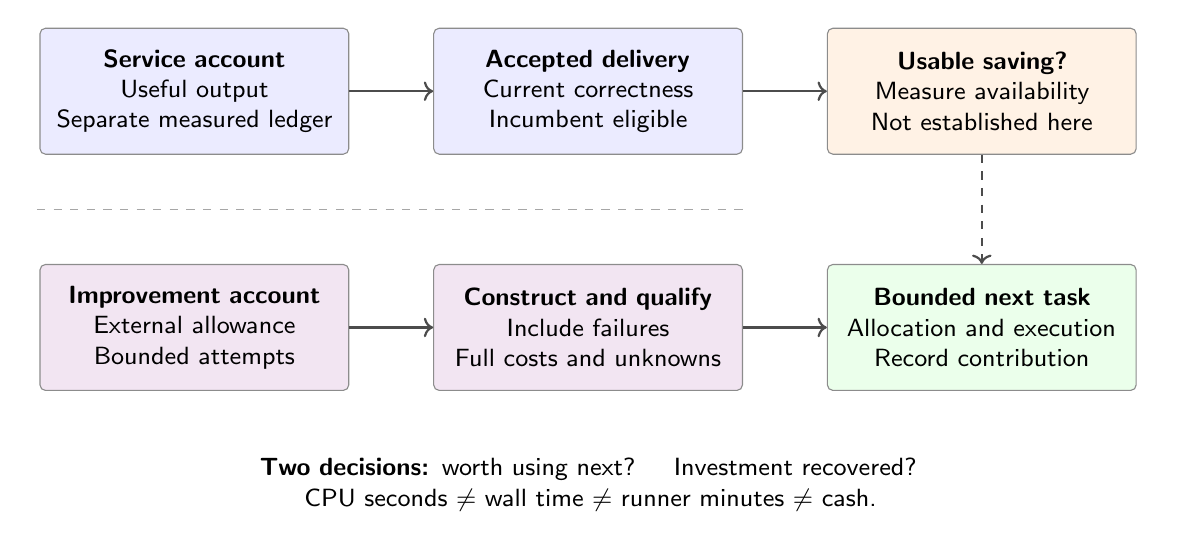
\begin{tikzpicture}[
 font=\sffamily\small,
 box/.style={draw=black!45,rounded corners=2pt,align=center,text width=3.5cm,minimum height=1.6cm,inner sep=6pt},
 flow/.style={->,thick,draw=black!70}]
\node[box,fill=blue!8] (service) at (0,0) {\textbf{Service account}\\Useful output\\Separate measured ledger};
\node[box,fill=blue!8] (delivered) at (5,0) {\textbf{Accepted delivery}\\Current correctness\\Incumbent eligible};
\node[box,fill=orange!10] (available) at (10,0) {\textbf{Usable saving?}\\Measure availability\\Not established here};
\node[box,fill=violet!10] (research) at (0,-3) {\textbf{Improvement account}\\External allowance\\Bounded attempts};
\node[box,fill=violet!10] (build) at (5,-3) {\textbf{Construct and qualify}\\Include failures\\Full costs and unknowns};
\node[box,fill=green!8] (next) at (10,-3) {\textbf{Bounded next task}\\Allocation and execution\\Record contribution};
\draw[flow] (service) -- (delivered);
\draw[flow] (delivered) -- (available);
\draw[flow] (research) -- (build);
\draw[flow] (build) -- (next);
\draw[flow,dashed] (available) -- (next);
\draw[dashed,draw=black!35] (-2,-1.5) -- (7,-1.5);
\node[font=\sffamily\small,align=center,text width=14cm] at (5,-5) {\textbf{Two decisions:} worth using next? \quad Investment recovered?\\CPU seconds $\ne$ wall time $\ne$ runner minutes $\ne$ cash.};
\end{tikzpicture}
\caption{Separate service, investment and feedback accounts. The dashed feedback path requires an actual usable-capacity witness, which this study does not establish. An externally supplied allowance remains external even when the preceding mission was faster. Separate measured accounts do not establish protected operational resource reservation.}
\label{fig:resources}
\end{figure}


We call the chain \emph{constructive succession} when an accepted parent is used to construct or qualify a distinct child that produces useful fresh outputs. We reserve \emph{net compounding} for an attributable positive net benefit across successive generations after their complete costs. \emph{Acceleration} additionally requires evidence of an increasing rate of qualified improvement, rather than a one-time speedup, repeated reuse or increasing cumulative output. The present finite trial cannot establish perpetual acceleration.

\section{The immediately usable browser journey}
\label{sec:browser}

The companion ships a self-contained HTML file and a modular version. Opening the single file requires no account, installation, wallet, API key or network request. The page runs through the existing unchanged \code{createWorkbench} implementation and its dependency closure. The adapter exposes the established seven-stage plan: Identify, Out-Learn, Out-Think, Out-Design, Out-Strategise, Out-Execute and Out-Evolve. The operation is local computation on disclosed public examples or permitted user-selected files.

The first visible example verifies a manifest of eight pinned source files. The next uses eight different gallery files, preserving the retained boundary. A third constructs a distinct drift report with deliberate changes, while the fourth refuses an unsafe path. The page exposes the user's goal, output, retained interface, correctness evidence, comparison and admission decision. These authored examples are explanatory demonstrations, separate from the Python confirmation instances and their measured results.

The research panel displays recorded evidence and says so. Browser operations do not run Git or reproduce Python CPU measurements. The connected-execution state explicitly remains unconnected: this study neither provisions a new credential nor reuses a held executor. The approved-executor demonstration required for an operational deployment remains outside the established evidence boundary. Jobs, Manager, Fleet and applicable token contracts contribute no executed live settlement utility to this trial.

STOP prevents further stage execution. Pause and inactive reopening preserve prior completed work without automatic restart. Export and restore bind the source identity and reject altered or mismatched evidence. Rollback retires a capability while preserving the completed mission history. Fifteen direct Node checks and 27 final actual Chromium checks cover the local and standalone entry points, downloads and readback, STOP, pause/resume, inactive recovery, tampered imports, selected files, refusal, rollback, keyboard navigation, no external requests and 390-pixel layout. An earlier 29-check browser receipt remains explicitly bound to its historical source. These checks establish the tested browser behavior, not an approved remote executor or a released production product.

\section{Limitations and the next falsifiable change}

The experiment is intentionally smaller than the ambition of an autonomously improving enterprise. The public code bodies are real, but confirmation repositories and archive defects are generated. Only one source ecosystem and one host are represented. Operating-system cache and external load are not controlled. Native Git tools and algorithmic templates are supplied by the research team. The study executes bounded construction and qualification, not a language-model agent discovering an unknown algorithm; it includes no equally capable language-model-agent trial.

The conventional constructor has the same content and budget as the flywheel. If they tie, the correct interpretation is ordinary reusable engineering value without an identified extra learning mechanism. If the specialist wins, it remains available as the incumbent. A reconstruction saving is conditional on the removed artifact and supplied knowledge; it is not proof that genealogy itself has productive value. Internal evaluator separation is I1 role separation, not organizationally independent or adversarially secure external evaluation~\cite[PDF p.~28]{neural_symbolic_v1}.

Full research expenditure and human effort are not measured. The trial cannot infer profit, investment recovery or monetizable GitHub minutes. The core browser works locally; existing release owners still control integration, qualification, merging and deployment. No source snapshot is treated as a live deployed-contract state and no draft or local result confers authority.

The next falsifiable design change should target a cost the present instrument actually leaves unresolved: diagnosis-to-repair selection on new package failure classes. A future predeclared trial could give every arm the same fastest reader, task information and conventional history, then compare a learned diagnostic policy against a mature direct fault-classification strategy. Its primary endpoint should be total effort to deliver a correct repair, including unsuccessful investigations and operator review. New protected cases and a new evidence boundary would be required. This paper does not launch that additional search or relabel its current cases as held out again.

\section{Conclusion}

The Software Capability Foundry delivers an executed source-verification improvement, a concrete reusable reader, and a content-bound construction path to a distinct archive-drift diagnostic. It keeps strong specialist tools, full correctness requirements, negative results and unknown costs in view. \ConclusionResult{} This is the practical standard for the next turn: retain what improves useful work, refuse unsupported reuse, and require fresh evidence before attributing a stronger improvement process to the system.

\appendix
\section{Reproduction and artifact map}

The complete companion contains source, executable asset bytes, exact source manifests, frozen configuration and analysis, public source-derived evaluation repositories, raw per-phase outputs, acceptance records, selected-execution traces, development attempts, independent internal-review records, browser downloads, LaTeX, bibliography and editable figures. The root \code{REPRODUCE.md} gives the exact commands. Reproduction should start in a new directory; the campaign refuses to overwrite an existing confirmation directory. A reproduction is labeled replication and retains the published cases. A new scientific confirmation requires a new prospective boundary.

\begin{longtable}{@{}p{0.31\textwidth}p{0.64\textwidth}@{}}\toprule
Location & Purpose\\\midrule\endhead
\code{src/} & Reader, constructor, drift comparison, worker, campaign, measurement and frozen analysis.\\
\code{protocol/} & Source boundary, selected method, budgets, environment and analysis rules.\\
\code{assets/reader/} & Retained executable parent and qualification metadata.\\
\code{development/} & Original and improved call-site timings, failed/superseded candidates, corrections and development acceptance.\\
\code{review/} & Independent specialist, protected generator, byte/drift oracles, adversarial checks and review.\\
\code{confirmation/} & Fresh generated repositories, archives, independent oracles and source provenance.\\
\code{results/} & Raw campaign, per-treatment phase outputs, acceptance bindings, analysis and cost account.\\
\code{browser/} & Self-contained HTML, unchanged workbench closure, local demo, tests and actual browser evidence.\\
\code{patches/} & Reviewable source-verification adaptations; not applied to production by the study.\\
\code{paper/} & Compilable manuscript, bibliography and editable TikZ diagrams.\\
\code{audit/} & Four-repository source audit, exact foundational-paper identities and mechanism crosswalk.\\
\code{publication/} & Explicit local/review/merge/deployment/public-access state and handoff.\\\bottomrule
\end{longtable}

\section{Claims and evidence boundaries}
\begin{longtable}{@{}p{0.29\textwidth}p{0.66\textwidth}@{}}\toprule
Claim & Required evidence and present interpretation\\\midrule\endhead
Useful optimization & Exact original outputs plus interleaved measured cost comparison on pinned A/B call sites. No full-CI or platform extrapolation.\\
Concrete retained asset & Executable bytes, version, contract, dependency/source identities, qualification, limits, maintenance unknowns and fallback.\\
Fresh usefulness & Protected byte/drift oracles on new generated instances, with all failures retained.\\
Actual parent use & Selected child execution calls the bound reader; trace identities independently match the accepted prior read.\\
Distinct successor & Reader returns committed bodies; child returns complete archive drift. Logic is bounded prewritten composition, not autonomous invention.\\
Improved improvement process & Requires a total-cost advantage over equally enabled conventional construction and strong direct tools; not inferred from lineage or outputs alone.\\
Investment payback & Requires full discovery, model, human, integration, storage and maintenance costs. Incomplete here.\\
Earned feedback & Requires actually usable freed capacity allocated to later work. A counterfactual CPU opportunity alone is insufficient.\\
Acceleration & Requires an increasing measured rate across independently qualified generations; unproved.\\
Operational/public status & Local execution, owner review, merge, release deployment and served-byte verification remain separate states.\\\bottomrule
\end{longtable}

\section{Research governance and disclosure}

This edition was developed with an interactive AI assistant and separate same-session roles for source audit, comparator/evaluator review and manuscript foundations. The specialist reader and byte/drift oracles were independently authored; all roles nevertheless share one organizational and computational context. Review separation is therefore internal, with source and task commitments for auditability. It is not external certification.

The benchmark makes no model-provider calls. That statement does not imply that research authoring was free: interactive model usage and human effort are unknown costs. Public repository inputs retain their applicable licenses. The new companion source is Apache-2.0; vendored files retain their original notices. Existing papers, prior negative results and source histories are preserved. Publication proceeds additively through the existing repository and coordination issue; no competing scheduler, production release owner or automatic-admission route is introduced.

\bibliographystyle{plainnat}
\bibliography{foundations}
\end{document}
